En este apartado se presentan los diagramas de Gantt que inicialmente se plantearon para el proyecto.

\begin{figure}[H]
    \centering
    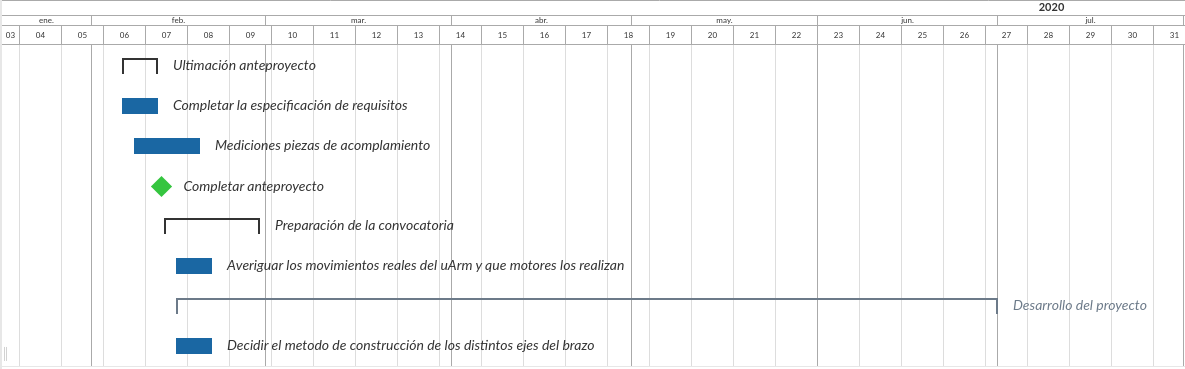
\includegraphics[width=1\linewidth]{pictures/DiagramaGanttGeneral.png}
    \caption{Diagrama de Gantt general}
    \label{fig:gantt_general}
\end{figure}

En el diagrama \ref{fig:gantt_general} observamos la planificación inicial del proyecto el cual tenia como fecha prevista de finalización el 30 de Junio.

Se pueden observar que, a nivel general, la planificación tenia 3 partes: El anteproyecto, La preparación para la convocatoria de soporte para el desarrollo de proyectos hardware y finalmente el desarrollo efectivo del proyecto.

\begin{figure}[H]
    \centering
    \includegraphics[width=1\linewidth]{pictures/UltimaciónAnteproyecto.png}
    \caption{Diagrama de Gantt del anteproyecto}
    \label{fig:gantt_anteproyecto}
\end{figure}

En el diagrama \ref{fig:gantt_anteproyecto} se desglosa la planificación del anteproyecto.

\begin{figure}[H]
    \centering
    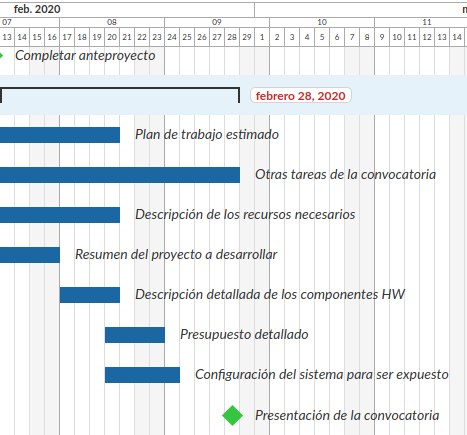
\includegraphics[width=1\linewidth]{pictures/PreparacionConvocatoria.png}
    \caption{Diagrama de Gantt de la preparación de la convocatoria}
    \label{fig:gantt_convocatoria}
\end{figure}

En el diagrama \ref{fig:gantt_convocatoria} observamos las distintas labores que se realizaron para completar el documento requerido. 

\begin{figure}[H]
    \centering
    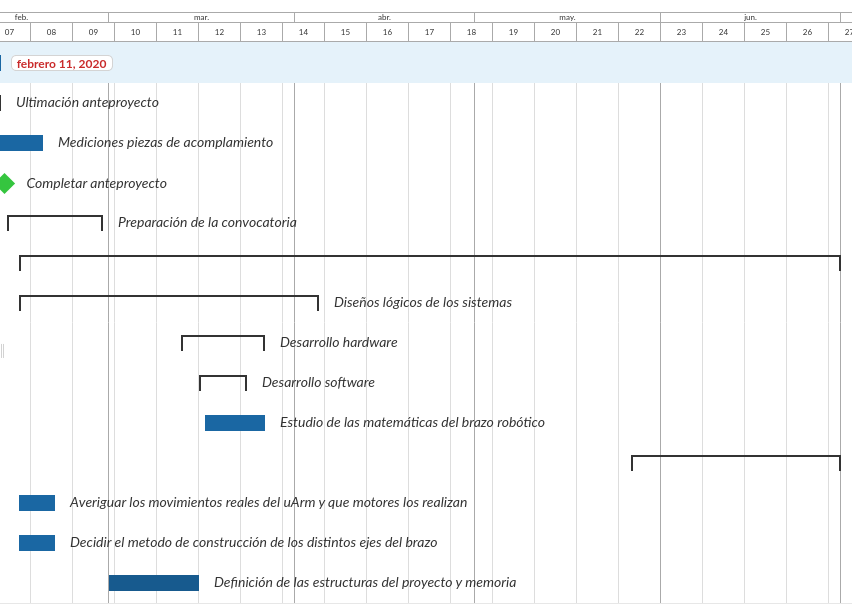
\includegraphics[width=1\linewidth]{pictures/DesarrolloProyecto.png}
    \caption{Diagrama de Gantt del desarrollo del proyecto}
    \label{fig:gantt_proyecto}
\end{figure}

En el diagrama \ref{fig:gantt_proyecto} se observa la planificación temporal de la parte técnica del proyecto.

La planificación temporal esta desglosada en varios otros subapartados que no son visibles en las imágenes \ref{fig:gantt_general},  \ref{fig:gantt_anteproyecto}, \ref{fig:gantt_convocatoria}, \ref{fig:gantt_proyecto}.

